\chapter{Background \& Objectives}

%This section should discuss your preparation for the project, including background reading, your analysis of the problem and the process or method you have followed to help structure your work.  It is likely that you will reuse part of your outline project specification, but at this point in the project you should have more to talk about. 



%\begin{itemize}
%   \item All of the sections and text in this example are for illustration purposes. The main Chapters are a good starting point, but the content and actual sections that you include are likely to be different.
   
 %  \item Look at the document on the Structure of the Final Report for additional guidance. 
   
%\end {itemize}

\section{Background}
\subsection{Introduction}

This project uses data and images collected during the course of experiments conducted at the National Plant Phenomics Centre (NPPC)\cite{_nppc}. The NPPC, based near Aberystwyth, houses a state-of-the-art, automated greenhouse and imaging system. During experiments, plants are housed on moving conveyors and are carried one by one through measurement chambers where images of various modalities (such as infra red and visible light) are captured from multiple angles. Physical and environmental measurements, such as plant weight, water usage or greenhouse temperatures, can also be captured automatically. More specific or specialist data (such as targeted phenotype or genotype traits) are captured following observation by staff at the facility.

The experiments at the NPPC are capable of investigating large sets of plants including whole breeding populations in order to inform how physical characteristics are affected by genes. Phenotyping experiments will often conduct a quantitative trait locus (QTL) analysis where sections of DNA corresponding to certain desirable phenotypes are identified, mapped and recorded for consideration in future breeding. The NPPC is capable of supporting a wide range of plants, from food-security critical cereal crops such as wheat and oats to plants that are promising sources of bio-fuel or biomass such as Miscanthus. The results of these experiments can directly affect the yield and robustness of future generations of important crops.

There is a wealth of data collected at the NPPC that is often never considered again following the conclusion of an experiment. This project seeks to provide an ongoing use for some of these data and images.

\subsection{Initial project topic}
The initial title for this project was `Building a plant Atlas from real images'.  In this context an Atlas is a term used to describe a visual reference for developmental stages within a subject of interest. Such an approach is commonly attributed to Tanner et al \cite{tanner_assessment_1975} for their work at numerically scoring the stages of bone development within the hands of infants and providing a visual reference for each stage. 

Biologists use numerical growth stage indices to chart the developmental milestones in the life cycle of a given plant. In cereals a popular scale for these growth stages is the 0 to 100 scale defined by Zadoks \cite{zadoks_decimal_1974} in 1974. These scales are often presented in an Atlas style with hand drawn, stylised images used to display detail of the characteristics of a particular growth stage. Figure~\ref{fig:bbch} shows an example taken from the BBCH scale which is based on the Zadoks cereal scale.

\begin{figure}[H]
    \centering
    
\includegraphics[width=\textwidth]{images/background/bbchscale}
    \caption{Example of `atlas' style visualisation of wheat plant development stages. Source : Wikimedia Commons \cite{bbch_scale}}
    \label{fig:bbch}
\end{figure}



 The aim of the original project was to utilise the images and data collected during a particular experiment at the NPPC in order to provide an atlas style visualisation using real plant images and providing a web based interface onto this visualisation with the intention of it being used as a reference for the biologists or a teaching aid and to sort or align the experiment population on growth stage and compare their physical characteristics. Further suggested work on this topic was to leverage some machine learning capability to attempt to draw conclusions or infer useful correlations from the datasets collected over the course of running experiments.

This topic was selected for the subject of this dissertation since it provided a chance at building a system that may have some practical use and application after the dissertation was complete. The topic also provided the opportunity to learn about certain plants, their life cycles and their importance as a research subject, this seemed like a more interesting problem domain when compared to other available choices.

\subsection{Change of project topic}

In the initial weeks of the project, meetings were arranged with Dr Roger Boyle, a researcher specialising in computer vision based applications at the NPPC. The purpose of these meetings was to discuss the direction and background of the originally proposed project and arrange visits to the NPPC itself in order to gain an understanding of the facility and its functions. Spike work, prototyping and research into plants, growth stages, atlases and investigations into agreement between expert opinions \cite{williams_comparing_1976} were the focus of these early weeks as opposed to investigations into the data being collected at the NPPC.

 In order for the original topic to be successful, the recording of key growth stage information during the course of an experiment was necessary, without these data points it would not be possible to build the proposed atlas visualisations. Unfortunately, where it was assumed that such data was being recorded as a matter of course during NPPC experiments, it became apparent that the recording of plant characteristics data during experiments was extremely sparse. When experiment data was provided for analysis it became clear that the approach to data collection was very different from what was expected. The interdisciplinary differences in attitude to data between the computer scientists and biologists involved was a key factor in the erroneous assumptions regarding the quantity and quality of collected data. The biologists who collect experiment data are often concerned only with growth stages which are directly associated with 
 
  

\subsection{Existing solutions}
%we looked mostly at zegami and the access-phenomics site, these were the similar systems that we researched primarily

Zegami, the site @ access.plant-phenoimics


\section{Analysis}
%Taking into account the problem and what you learned from the background work, what was your analysis of the problem? How did your analysis help to decompose the problem into the main tasks that you would undertake? Were there alternative approaches? Why did you choose one approach compared to the alternatives? 

%There should be a clear statement of the objectives of the work, which you will evaluate at the end of the work. 

\subsection{Requirements}

%In most cases, the agreed objectives or requirements will be the result of a compromise between what would ideally have been produced and what was felt to be possible in the time available. A discussion of the process of arriving at the final list is usually appropriate.
\begin{itemize}
\item \textbf{Web based system}
\item \textbf{Integrate with NPPC data repository}
\item \textbf{Browse plants and plant images}
\item \textbf{Add meta data to plants and plant images}
\item \textbf{Import experiment data}
\item \textbf{Display graphs of data in system}
\item \textbf{Administrator panel or page to manage the system}
\end{itemize}







\subsection{User Roles}
For this system there were two identified user roles

\begin{figure}[H]
    \centering
    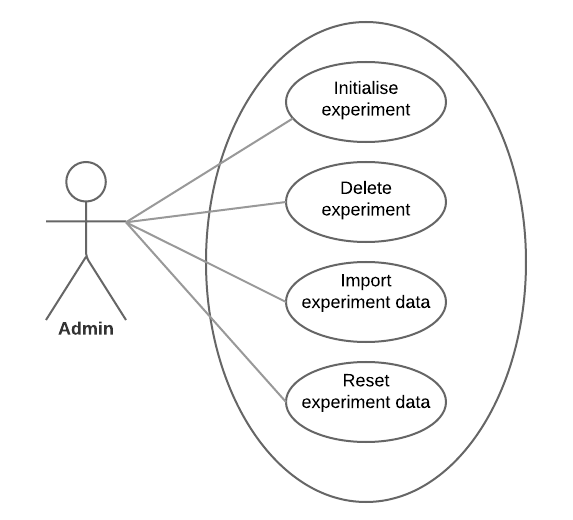
\includegraphics[width=0.5\textwidth]{images/analysis/admin_case}
    \caption{Use cases for admin user}
    \label{fig:admin_case}
\end{figure}
\begin{figure}[H]
    \centering
    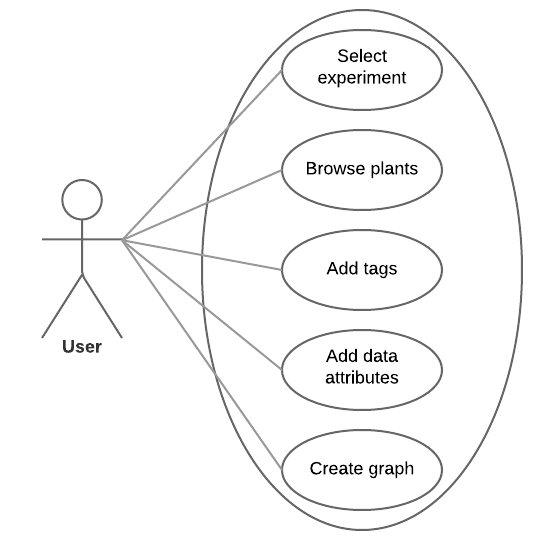
\includegraphics[width=0.5\textwidth]{images/analysis/user_case}
    \caption{Use cases for generic user}
    \label{fig:user_case}
\end{figure}

\section{Process}

Plan driven approaches traditionally associated with software development projects usually expect that all system requirements are understood and collected prior to any further work on design or implementation. A number of factors made such an approach unsuitable for this project, chiefly a lack of domain knowledge made up-front requirement gathering difficult and the requirements themselves were likely to be poorly defined and subject to change. 

The methodology used for the delivery of the project was an agile approach based on the popular SCRUM methodology. For the duration of the project, work would be carried out in time-boxed iterations or `sprints', each a week long. Sprints would begin with a planning session and end with a release of the system software. At the conclusion of each sprint a short retrospective analysis of the sprint would take place, looking at what went well and what could improve for the next iteration. The focus on incremental delivery of working software allowed the project to evolve in an emergent fashion whilst remaining continuously functional as features were prototyped, designed and implemented.  

System requirements were broken down into user stories which in turn were broken down into individual tasks if necessary. As in SCRUM, these stories were held in a backlog until being added into a current or future sprint depending on priority and the goal for a particular sprint. Emergent issues such as priority bugs could easily be incorporated into the wider context of the current sprint if necessary which allowed work to be focused on the most pressing issues. The Jira \cite{jira} issue tracking application was used in support of this process providing an environemnt in which to specify and track user stories,task and sprints, see section~\ref{jira_sec} for further details. 

During a sprint, each day would begin with a quick overview of tasks in the sprint, replicating the `stand-up' meetings common in SCRUM. Work would be commenced or continued on the task deemed highest priority at the time. At the end of each day a short update would often be posted on the project blog available at \url{https://siongriffithsblog.wordpress.com/} summarising the days activity. The blog itself has proven to be a useful part of the process, helping to document certain aspects of the implementation and design that may have otherwise been forgotten.


\subsection{Time Management}
Effective management of time is a key consideration of any reasonable development process model. Partway through the project it was decided to fully adopt the Pomodoro technique \cite{pomodoro}, working in blocks of twenty five minutes with complete focus on the task at hand, referred to as Pomodoros. A five minute break is taken after each successful twenty five minute work block in order to avoid the mental fatigue of attempting to remain focused and productive for an extended amount of time. Taking these regular, short breaks allowed for a higher degree of productivity over the course of a work day.

Having distinct blocks of time in which to complete work compliments the SCRUM approach to effort tracking and estimation. Although not part of the initial process, towards the latter half of the project after gaining a sufficient feel for the possible output of a single Pomodoro, all work was estimated in terms of the Pomodoros required to complete the task. The goal for a given sprint was to achieve sixty Pomodoro and use this figure as the budget for work that could be done. It was fairly difficult to estimate in terms of Pomodoro and often fairly inaccurate, although the productivity aspect certainly works, the more abstract and popular `story-point' method of effort estimation is what would be used if the project was repeated.

Figure ~\ref{fig:pomo1} shows the early Pomodoro tracking during two iterations. A successful Pomodoro would result in a sticker being allocated to that day. It was preferable to have Pomodoro goals for a given sprint rather than concrete work times (for example nine-to-five) since this allowed a great deal of flexibility whilst also maintaining that a weeks worth of work was to be done. Effort could be expended in the beginning of the week in order to have more time later on for example.  

\begin{figure}[H]
    \centering
    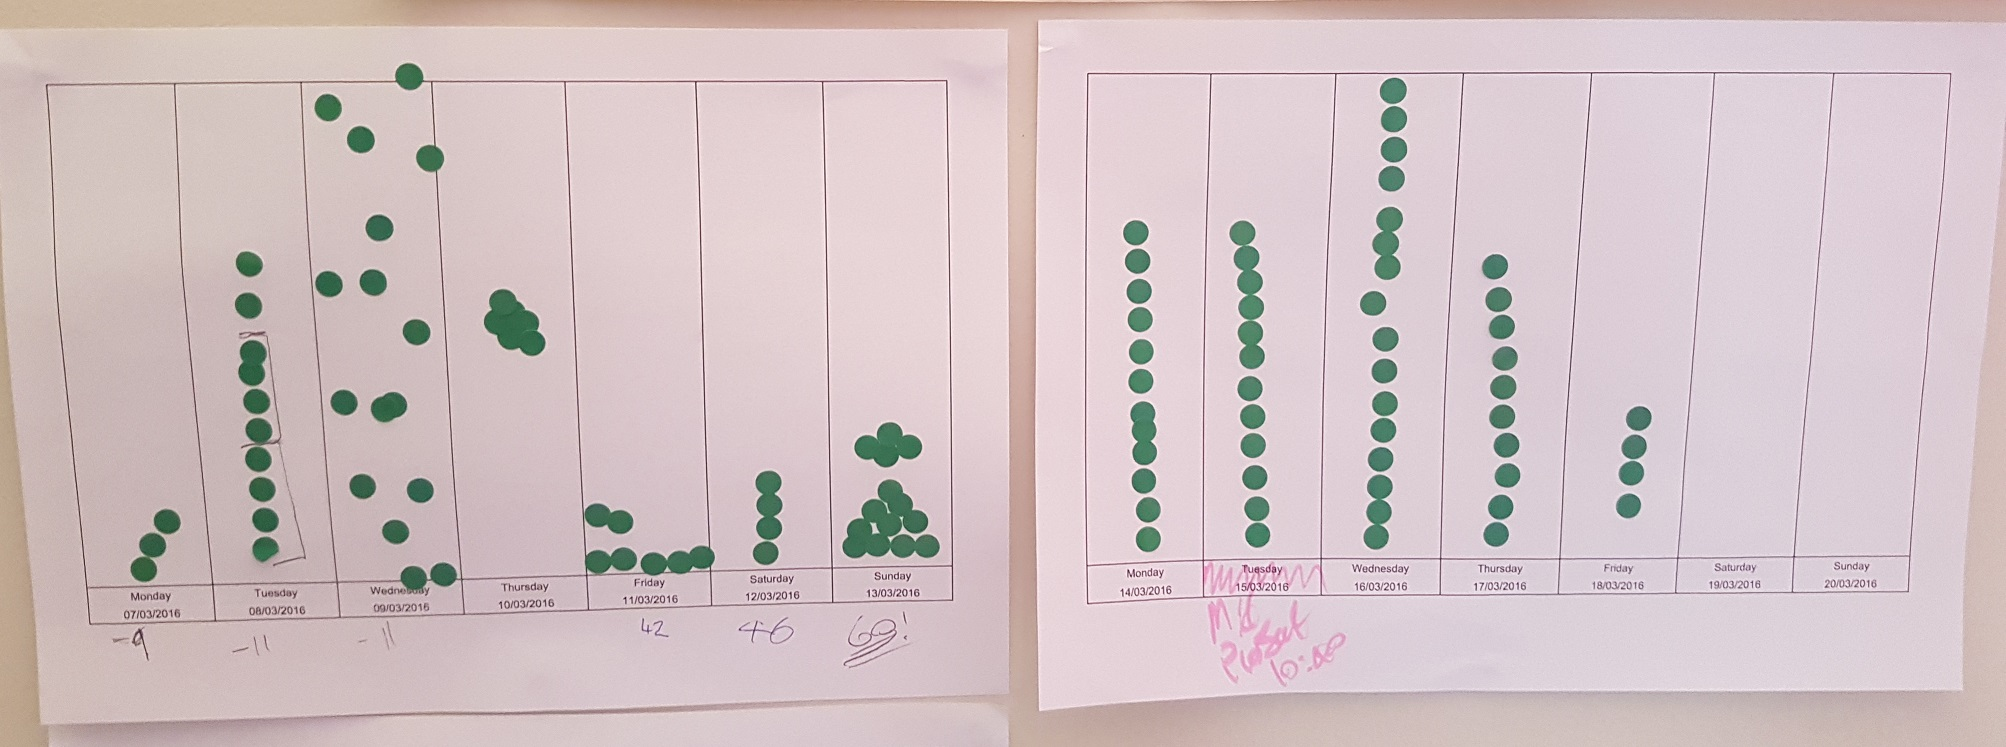
\includegraphics[width=\textwidth]{images/process/pomotrack}
    \caption{Tracking pomodoros}
    \label{fig:pomo1}
\end{figure}


%The process used for the project was an agile based approach similar in style to Scrum although adapted for a project team of one. The process centred around User Stories and short iterations of one week. 

